
\begin{figure}[!ht]
       \centering
        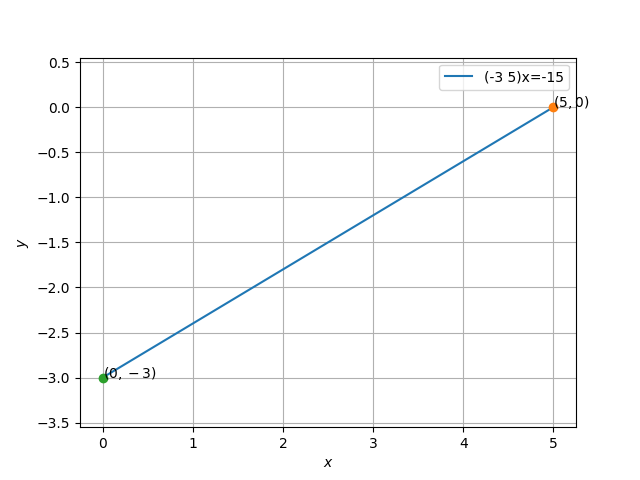
\includegraphics[width =\columnwidth]{line.png}
        \caption{Required plot of the line $\myvec{-3 & 5}\vec{x}=-15$ }
        \label{5/4/fig:Line}
\end{figure}
From the given information, 
\begin{align}
\vec{m}=\myvec{1\\m}\implies\vec{m}=\myvec{1\\\frac{3}{5}},c=-3
\end{align}
Hence, the normal vector of the line is
\begin{align}
\vec{n}=\myvec{\frac{-3}{5}\\1}
\end{align}
Equation of the line is
\begin{align}
\vec{n}^{T}\vec{x}&=c
\\
\implies \myvec{\frac{-3}{5}&1}\vec{x}&=-3
\end{align}
Fig.\ref{5/4/fig:Line} is the plot of the line.


